\def\myname{Mihai $B\hat{a}ce$}

\title{Automatic Depth Camera Calibration\\
    \large Semester Project}
    
\author{
  {\emph Author:} Mihai Bace \\
  \texttt{mihai.bace@epfl.ch}
  \and
  {\emph Supervisor:} Julien Pilet \\
  \texttt{julien.pilet@aptarism.com}
  \and
  {\emph Supervisor:} Vincent Lepetit \\
  \texttt{vincent.lepetit@epfl.ch}
}

\date{\today}
\documentclass[a4paper,11pt]{report}
\usepackage[utf8]{inputenc}
\usepackage{graphicx}
\usepackage{url}
\usepackage{hyperref}
\usepackage{amsmath}
\usepackage{mathtools}
\usepackage{listings}
\usepackage{lstautogobble}
\usepackage[margin=1in]{geometry}
\usepackage{caption}
\usepackage{xcolor}

\lstset{basicstyle=\ttfamily,
  mathescape=true,
  escapeinside=||,
  autogobble}
  
\begin{document}
\maketitle

\tableofcontents

\begin{abstract}

The purpose of this report is to present a method in which a normal RGB camera can be calibrated using a 3D camera. The 3D camera used for calibration is a Microsoft Kinect which has depth detection capabilities using an infra-red sensor. Using the Kinect, this report will present an approach to calibrate a normal camera based on image processing techniques. The calibration approach is based on collecting a set of corresponding points from the Kinect depth image and the normal camera RGB image using a pattern. The pattern used in this report is a cone with a green colored tip. In order to detect the pattern, this report will describe techniques as color filtering, subtracting two consecutive Gaussian blurs and template matching. 
\end{abstract}

\chapter{Introduction}
The purpose of this project is to accurately calibrate a non 3D camera using a 3D camera. In this report we try to calibrate a normal camera (e.g.) using a Microsoft Kinect. \\

\section{About the Kinect}

The Kinect is a motion sensing device, initially built as an add-on for the Microsoft XBOX 360 gaming console, but later on ported to the PC. It is a relatively inexpensive device that incorporates a lot of different sensors like an RGB camera, a depth sensor and a multi-array microphone which provide full-body 3D motion capture [Wikipedia]. The depth sensor is a combination of an infrared laser and a monochrome CMOS sensor which can capture 3D data under any lighting conditions. \\
The sensors being used for this project are:

\begin{itemize}
	\item RGB camera
	\item Depth sensor: monochrome CMOS and infrared laser
\end{itemize}

\noindent
The RGB camera can capture 8-bit images at a VGA resolution (640 x 480 pixels). However, the hardware is capable of capturing images at higher resolutions (1280 x 1024 pixels), but at a lower frame rate. The frame rate for video capture from the RGB camera can vary between 9 Hz and 30 Hz.
\\
The second sensor used, the depth sensor, is very important for the 3D sensing capabilities of the device. The monochrome camera can capture images at VGA resolution (640 x 480 pixels) with 11-bit depth, which can assure 2,048 levels of sensitivity. The sensor has a practical range between {\bf 1.2 meters} and {\bf 3.5 meters}. In order to be able to take advantage of the Kinect's motion sensing abilities an area of 6 $m^2$ is needed. 
\\
The Kinect connects to the PC or XBOX using a USB interface, but it requires an additional power supply due to the motorized tilt mechanism. 
\\
Since its launch, the Kinect has attracted a lot of interest from developers and as a result, Microsoft has decide to release and SDK for Windows in the spring of 2011. The SDK is compatible with Windows 7 and newer versions and it allows developers to build applications with {\bf C++, C\# or Visual Basic} in combination with the IDE called Microsoft Visual Studio (version 10 or newer). 
\\
Some of the features of the SDK are the following [Wikipedia]:
\begin{itemize}
	\item Raw sensor streams: Access to low-level streams for the depth sensor, color camera sensor and the microphones
	\item Skeletal tracking: The capability to track one or two people based on the skeleton and use this information for gesture driven applications (e.g. games, medical applications etc.)
	\item Audio capabilities: Audio processing capabilities include echo cancellation, acoustic noise suppression and the very interesting speech recognition
	\item Sample code and documentation: a very good starting point for all the beginners who want to develop applications using the Microsoft Kinect
\end{itemize}

\noindent
For those who are interested to develop applications for the Kinect, the latest SDK (at this date) is Microsoft Kinect SDK 1.7 and it can be found at the address below:

\url{http://www.microsoft.com/en-us/kinectforwindows/develop/developer-downloads.aspx}

\noindent
Since the Kinect has been received with a lot of enthusiasm by the developers, there are some 3rd party libraries and drivers that can be used. Some of the most famous ones are:
\begin{itemize}
	\item OpenNI \url{http://www.openni.org/}
	\item libfreenect, part of the Open Kinect project \url{http://openkinect.org/wiki/Main_Page}
\end{itemize}

\section{Depth camera calibration}
\noindent
The depth camera calibration is a process in which we try to reproject a 3D point to a 2D point captured by the normal RGB camera. Without a calibration this would not be possible. The calibration helps to accurately detect what 2D point from the RGB image corresponds to what 3D point (in our case detected by the Kinect).

\section{Motivation of this project}
\noindent
The process in which a 3D point is reprojected to a 2D image is not new. Depth camera calibration has been done before, but this process implies to manually find a minimum number of correspondences. Two points are valid points for the set of correspondences if the points in the 2D image and the 3D image represent the same physical point (pixel in the image plane). Once the points have been found, we try to estimate the calibration matrix using a model. Based on this model all the other points will be reprojected and thus the calibration is completed.  
\\
\noindent
Finding the correspondences between the 2D image and the 3D image is a tedious work and it implies a lot of time. This is why an automatic depth camera calibration would be useful. By having an automatic way to detect the correspondences, the user only needs to walk with a template in front of the camera and the "good" points will be selected automatically. What exactly are good points? We will describe this in the following chapters. 
\\\\
\noindent
This document will describe in the following chapters a way in which the automatic depth camera calibration can be achieved. The design chapter describes the process from the algorithm point of view, what methods we have used and why. The implementation chapter will go into more implementation details and will describe the functions that make the algorithm work. In order to be able to asses our results, we need some visualization tools. Chapter 4 will describe the visual interfaces. The 5th chapter will present the final result, the calibration.    


\chapter{Design}
\noindent
This chapter will describe the steps of the algorithm that we have designed. Each step will be described in detail and with pictures which will help better understand.
\\
For the automatic depth calibration of the camera we must find a set of equivalent points in different images, also known as correspondences. This means that if we identify a point in the image from the Kinect, we must find its equivalent in the image provided by the normal camera. In order to do this, we have created a pattern that we would like to detect. 
\\\\
The pattern that we want to detect is in the shape of a cone with its tip colored green. The color of the tip is not important, the algorithm can be adapted to work with almost any color. For experimental purposes, we have decided to keep the color of tip green. 
\\
An image of the pattern can be seen below:

$$ <Image of pattern> $$

\noindent
The algorithm that we describe in this report depends on the pattern that we have chosen. Similarly, it could be adapted in the future to work with different patterns, but we believe that the pattern that we have chosen is easy to build and it provides good results. 
\\\\
The steps for calibration are the following:
\begin{enumerate}
	\item Get the depth map from the Kinect
	\item Get the RGB image from the Kinect
	\item Get the RGB image from the webcam
	\item Perform color filtering on the webcam RGB image
	\item Perform color filtering on the Kinect RGB image
	\item Perform filtering on the depth map based on the Kinect RGB color filtering 
	\item Apply the Gaussian blur on the webcam RGB image and do the difference between two Gaussian blurs
	\item Apply the Gaussian blur on the Kinect RGB image and do the difference between two Gaussian blurs
	\item Pattern detection: Do template matching on the depth image
	\item Pattern detection: Do template matching on the webcam RGB image
	\item Pattern detection: Do template matching on the Kinect RGB image
	\item When all three templates have been matched, we have obtained a set of correspondences
	\item Add the correspondences to the calibrator
	\item Perform an iterative calibration and eliminate outliers
	\item Display the Kinect depth map recolored from the webcam RGB image 	
\end{enumerate}

\section{Get the depth map from the Kinect}
\noindent
One of the first steps in any image processing application is to get the images/data that we need for further processing. In our project, the first step is to obtain the depth map provided by the Kinect. Each frame is being captured and stored as an image. Each pixel in the image holds the depth information of that pixel. The depth information can be extracted and we can obtain the depth in millimeters.
\\
For accuracy, the depth map will be stored exactly the way it is received from the Kinect. An example of such an image can be seen below. The completely black pixels show a depth of 0 millimeters. This means that the Kinect cannot obtain any depth information for those pixels. Points that are gray or close to black are the points that are close to the sensor, while points that are far away are white or closer to white. 

$$ < depth image > $$

\section{Get the RGB image from the Kinect}
\noindent
Once the depth map has been obtained, we must obtain the RGB images from the Kinect and from the normal camera, the webcam. The image from the webcam is also captured frame by frame, it is an image of 640 x 480 pixels. Each point (pixel) stores information about the 3 channels, red, green and blue. 
\\
A sample of the image captured by the webcam can be seen below.

$$ < RGB image > $$

\section{Get the RGB image from the webcam}
\noindent
Just like in the previous step, we must also get the RGB image from the Kinect's RGB camera. The process is the same as in the previous step, with a small difference that every point (pixel) stores 4 channels (BGRA), not 3 like in the previous case. 
\\ 
A sample of the image can be viewed below. 

$$ < Kinect RGB Image > $$

\section{Color filtering on the webcam RGB image}
\noindent
As described in the beginning of this chapter, our goal is to be able to identify a specific pattern. Once the pattern has been detected we can select the center of the pattern and consider a point to which we need to find an equivalent. 
\\
In the sections described below, we will perform template matching on the 3 images that we have obtained previously. Since template matching is not very accurate in all situations, we must find a way in which we can focus our "attention" to only a part of the image and not to the whole image. 
\\
We have identified that performing a color filtering on the RGB images, the result of the template matching (described in the sections below) is greatly improved.
\\
Color filtering is a process in which we filter the RGB image based on a specific color, or a specific range. We know that the tip of our pattern (the cone) is green, so we need to filter out of the image everything that is not green. Once all the points that are not green are filtered from the image, we can try to identify which green area represents the tip of our cone. 
\\
Color separation is quite difficult on the RGB image, so we must first convert the image to the HSV color space. The HSV color space is represented by hue, saturation and value. This allows for a much better segmentation of the image based on the color features. The filtering is easily achieved using the OpenCV function, \emph{cv::inRange}. 
\\
The result of the \emph{inRange} function provided by the OpenCV is a matrix that stores 0 where the color has not been found and 255 where the color of that pixel was in the range specified. Based on this result, we need to compute the center of the color that we have detected. We can do this by computing the median x-axis coordinate and the median y-axis coordinate. This can approximate the position of the peak. Once we have determined the peak we create a window of 100 x 100 pixels which will represent our region of interest. 
\\
An image of the mask can be viewed below.

$$ <image of mask> $$

\noindent
An image of the RGB image filtered by this mask can be viewed below.

$$ <image of mask> $$

\noindent
As we can observe, the accuracy of the color filtering is very good and the region of interest is exactly what we are looking for. The result of this step will be the input to the next step, where we will apply several times a Gaussian blur on the filtered image. 
\\\\
From an implementation point of view the range of the HSV space for which the color filtering is done is the following

$$ From \; cv::Scalar(38 , 100 , 100) \; To \; cv::Scalar(75 ,255 ,255 ) \; $$

\noindent
The resulting image of this step has the same characteristics as the input image, with the following differences. The resolution is still 640 x 480 pixels, the type of the image is {\bf CV\_8UC3}, but we can only see the image though the window provided by the mask. The rest of the image is black. 

\section{Color filtering on the Kinect RGB image}
\noindent
Color filtering on the Kinect RGB image is done in an almost exact way as the one described previously. The only difference comes from the fact that the Kinect RGB camera is different from the webcam and the color range is also different. 
\\
The range that we have used for the \emph{inRange} function is the following:

$$ From \; cv::Scalar(38 , 110 , 110) \; To \; cv::Scalar(75 ,255 ,255 ) \; $$

\noindent
The resulting image is {\bf CV\_8UC4}, since the input image also stores information on 4 channels. 

\section{Filtering on the depth map}
\noindent
Now that both RGB images have been filtered using a color mask, we also need to filter the depth map. Actually, filtering the depth map is more important than filtering the RGB images. Doing template matching directly on the depth image (each pixel stores the depth in millimeters) can lead to a lot of false positives. The shape of the cone can be easily found in other places, for example the shape of a leg, or a pillow or different objects that can influence the detection. 
\\
Performing a color filtering on the depth map is not really possible since there is no color information. So how can the filtering be achieved? Well, first of all, we have filtered the Kinect's RGB image and we have determined the center of the region of interest. We also know that the Kinect's depth sensor and RGB sensor are calibrated, so we could be able to see which point from the depth image corresponds to the point from the RGB image. 
\\\\
This is quite an easy task to achieve using the SDK provided by Microsoft. We just have to scan the depth map and see each of the depth map's pixel equivalent in the RGB image from the Kinect. The function that does this is 

$$ NuiImageGetColorPixelCoordinatesFromDepthPixelAtResolution $$

\noindent
and it takes as input the resolution of the two images (640 x 480 pixels), a 3D point (current point in the scan through the depth map) and it returns an $X$ and $Y$ coordinate which represent the location of the point we are looking for in the RGB image. 
\\
Once this point has been found, we also apply a mask of 100 x 100 pixels and this way we get our region of interest. 
\\\\
The region of interest after filtering can be seen below:

$$ <filterRegionOfInterest> $$

\section{Apply Gaussian blur to the webcam RGB image}
\noindent
Once that we have found the region of interest for our pattern, we need to be able to detect it. The RGB image itself does not provide a lot of information, so we have to further process it. A good way in which we can identify the peak of a cone is by apply a Gaussian blur to the image, applying the Gaussian blur again and then performing the difference between the two images with Gaussian blur. Before applying the Gaussian blur we have to convert the image to gray scale.
\\
The Gaussian blur can be applied using the OpenCV function \emph{cv::GaussianBlur} and we need to specify the input image, the output image and the size of the kernel. 
\\\\
We first apply a Gaussian blur with a kernel size of 21 x 21 pixels. We then apply a Gaussian blur of 21 x 21 pixels. We subtract the two images and we obtain one image where we can observe the peak of the cone. We can notice that it represent a disc like shape with large values, representing a local maximum. Since we have already done color filtering, it is easy to observe that it is the only disc shaped maximum (white disc) in the image, more specifically in the region of interest.
The result of this step can be seen in the image below.

$$ <differenceBetweenTwoGaussianBlurs>$$

Another important aspect in this step is obtaining an output image as precise as possible. As a result, we first convert the input images which is {\bf CV\_8UC3} to gray scale and then to {\bf CV\_32FC1}. With floating point values we get much better precision and this will be useful for the next steps where we perform template matching to detect out pattern. 

\section{Apply Gaussian blur to the Kinect RGB image}
\noindent
The process of apply a Gaussian blur to the Kinect RGB image is exactly the same as the one for the RGB image for the webcam. The only difference is the size of the second kernel for the second filtering. It is no longer a 21 x 21 pixels kernel, it is 35 x 35. The value for this kernel has been found empirically. 
\\\\
Just like in the previous case, for greater accuracy, the resulting image will be {\bf CV\_32FC1}.

\section{Pattern detection: template matching on the depth image}
\noindent
Now that all the preprocessing has been done, we can perform template matching to find the pattern that we are looking for. In order to perform template matching we must first select a template. This is done manually and it is read from a file. The size of the template varies between 30 to 60 pixels, depending on the size of the pattern and the range we want to detect it in. 
\\\\
Template matching is done using OpenCV's function \emph{matchTemplate} and it takes as input the depth image, the template for the depth image and the way in which it will evaluate the result. In our project we have chosen \emph{CV\_TM\_CCOEFF\_NORMED}. This means that in the result of the template matching, the best match will be the point with the maximum value in the image. A value of 1 means a perfect match, while a value of 0 means that the area tested and the template are completely different. 
The template matching will return a point, the left top corner of the match (the template has a square shape). To determine the center of the area where the matching was best we just take the point returned by the template matching function and we add half the size of the width or height of the template. 

$$ depthMatchPoint->x = matchLoc.x + depthTempl.cols/2 $$
$$ depthMatchPoint->y = matchLoc.y + depthTempl.rows/2 $$

\noindent
In order to be sure that the template has been successfully detected we also apply a threshold on the result. Thus, in order to have a valid match, the value returned by the function must be over $0.8$. 
\\\\
Template matching works good, but it is not reliable if the position on the pattern changes in the real world (if the pattern is further away or closer to the camera). When the pattern is far away from the camera, the pattern seems small. To overcome this issue we have used one of OpenCV's functions called \emph{cv::pyrUp} which doubles the width and the height of the initial image. This way, the image is bigger and the pattern is also bigger, so it can be matched with the original template. 

\section{Pattern detection: template matching on the webcam RGB image and Kinect RGB Image}
\noindent
In order to detect the pattern that we have created we also do template matching on the RGB image from the webcam. The template matching process is the same as the one described before. The difference comes from the fact that the template is different. The template is taken from the result of applying to consecutive Gaussian blurs and subtracting them. 
\\
The template matching will return the center point of the template, where the template matches best the current frame. Also the thresholds are different. The template matching on the RGB images are more accurate, so a threshold of $0.75$ is enough to get a good result. 

\section{Validation of template matching}
\noindent
Once the template matching has been performed on the tree images (the depth map, the RGB image from the Kinec and the RGB image from the webcam) we must make sure that the points returned are valid. 
\\
We cannot verify the point from the RGB image of the webcam, but we can check the points provided by the two sensors of the Kinect. This is done using the Kinect calibration. 
\\\\
We use again the function from the Kinect SDK:

$$ NuiImageGetColorPixelCoordinatesFromDepthPixelAtResolution $$

\noindent
and we provide as input the point returned by the depth template matching. The result will be a point $P(x, y)$ which corresponds to a point from the RGB image of the Kinect. We take the point returned from the RGB template matching from the Kinect and we calculate the Euclidean distance between them. If the distance is greater than a certain value (in practice this value is set to 8 pixels), the points are considered to be a bad match. Otherwise we consider the points to be valid and we will feed them to the calibrator. 

\section{Add correspondences to the calibrator}
\noindent
We now have successfully identified the patterns in all three images and we must calibrate the webcam. 
\\\\
The calibrator has been provided by Julien Pilet, one of the supervisor of this project. The calibration gathers a set of correspondences (a point from the RGB image from the webcam and a point from the depth map) and after enough points have been gathered we try to calibrate the camera. The result of the calibration will be a calibration matrix which can later be used to reproject any point from the depth image to the RGB image. 
\\\\
However, it can happen that the points which have been identified as correct correspondences are actually outliers. A set of points are considered to be outliers if after we reproject the point, the Euclidean distance between the reprojected point and the detected point (from the RGB webcam image) is greater than a certain value. These outliers need to be eliminated because they make the calibration error to be large. 
\\\\
In short, the calibrator is fed with the following points:
\begin{itemize}
	\item depthMatchPoint: P(x,y,z) - a point which has been correctly identified using the template matching technique. The point comes from the depth map of the Kinect.
	\item rgbWebcamMatchPoint: R(x,y) - a point which has been correctly identified using the template matching technique on the RGB image from the webcam. 
\end{itemize}  

\section{Iterative calibration and outliers elimination}
\noindent
As mentioned in the previous case, the first try to calibrate the camera can lead to quite a large error (in practice this error can be between over 20 pixels). This error is large and it will not lead to a good calibration. In order to improve the calibration we must identify which of the points discovered are actually outliers and we need to eliminate them and recalibrate the cameras. 
\\\\
The process of removing the outliers is described below:
\begin{itemize}
	\item Calibrate the camera
	\item Get the projections from the RGB image and the 3d points from the depth image
	\item Reproject all the 3d points
	\item Let's consider P a point from the projections and P' its reprojection using the calibration. If the Euclidean distance between them is larger than a value, we remove this point.
	\item Recalibrate the cameras without the outliers
	\item Repeat the whole process until the reprojection error is minimum.
\end{itemize}

\noindent
What does a minimum reprojection error mean? It can happen that one bad point influences all the other points in the calibration. Taking this into account, we cannot try to remove all the points with a starting error very small. As a result, the iterative calibration considers an error of 1000 pixels. This is a very large value, but it does not change the future outcome. After the outliers which have an error of over 1000 have been eliminated, the error is halved (500 pixels) and the process repeats. The iterative calibration process repeats until we get an error below 2 pixels. 

\section{Depth color reconstruction based on the calibration}
\noindent
Now that we have a calibration and an acceptable error we need a way to visualize the final result of this project. One way to do it is to try to recolor the depth image based on the RGB image from the Kinect. Wihtout a calibration, this process would be impossible since we do not know which points from the depth image correspond to which points from the RGB image of the webcam.
\\\\
With the calibration, we scan the depth map and we reproject each 3D point to get its equivalent from the RGB image. The point from the depth map is colored based on the equivalent point from the webcam's image. 
\\
The result of a depth color reconstruction looks like in the image below.

$$ <depthColorReconstruction> $$   


\chapter{Implementation}
\noindent
This chapter will describe the technologies behind this project, the reason why we have chosen them and some of the most important functions in the implementation. 
\\\\
This project has been implemented in {\bf C++} using {\bf OpenCV, OpenGL and the Kinect SDK}. OpenCV has been used for the image processing part of the project, the Microsoft Kinect SDK has been used to obtain the data from the Kinect and OpenGL has been used to be able to produce a 3D point cloud of the depth map and recolored using the calibration. Based on this categorization, I will describe some of the most important functions from the implementation of this project. 

\section{Microsoft Kinect SDK}
\begin{itemize}
	\item \textcolor{blue}{HRESULT initKinect()} - This function initializes the Kinect's sensor and opens the streams for both RGB image acquisition and depth image acquisition. 
	\item \textcolor{blue}{void getKinectPackedDepthData(USHORT * dest)} - It returns an array of the size $width \times height$ (of the image) with the information captured from the Kinect's depth sensor. It is important to note that each value is not the value in millimeters, it is a Microsoft specific format. The depth information in millimeters can be extracted using the function \emph{NuiDepthPixelToDepth}.
	\item \textcolor{blue}{cv::Mat getDepthImageFromPackedData(USHORT * data)} - Returns an array like in the previous function, but with the depth information in millimeters. 
	\item \textcolor{blue}{void getKinectRGBData(BYTE * dest)}  - Returns an array with the RGB information from the Kinect. 
	\item \textcolor{blue}{float getDepthInMeters(USHORT * data, int x, int y)} - Return the depth in meters of a specific pixel from the depth map. 
\end{itemize} 

\noindent
As we can see, these functions are used for data acquisition. The arrays returned by these functions will be converted to OpenCV specific structures, \emph{cv::Mat}. 

\section{Image Processing - OpenCV}

\begin{itemize}
	\item \textcolor{blue}{void loop()} - The main loop of the program. All the steps required for the processing and the display are put together here.  
	\item \textcolor{blue}{cv::Mat getColorMask(cv::Mat inputImg, int w, int h, string window\_name, cv::Scalar min\_color, cv::Point * median)} - Returns a CV matrix which holds the color mask to filter an image. 
	\item \textcolor{blue}{cv::Mat filterImageByColor(cv::Mat inputImg, cv::Mat maskImg)} - Returns the filtered image based on the mask obtained from the previous function. 
	\item \textcolor{blue}{bool getDepthPointFromRGB(cv::Mat depthImg, USHORT * data, cv::Point rgbPoint, cv::Point * newPoint)} - Given a point from the RGB image it returns the equivalent point from the depth image based on Kinect's calibration. 
	\item \textcolor{blue}{bool getRGBPointFromDepth(cv::Mat rgbImg, cv::Point depthPoint, USHORT * data, cv::Point * newPoint)} - It returns the RGB point from the Kinect's RGB image given as input a depth point from the depth map.
	\item \textcolor{blue}{bool checkPoints(cv::Point a, cv::Point b, int threshold)} - Verifies if the Euclidean distance between two points is larger than a threshold. 
	\item \textcolor{blue}{float getDistance(Point2f p1, Point2f p2)} - Return the Euclidean distance, measured in pixels, between two points. 
	\item \textcolor{blue}{void removeOutliers(Point2DVector * projections, Point3DVector * points3D, Point2DVector reprojections, float error, vector<int> pointIds, Point2DVector * newProjections, Point3DVector * newPoints3D, vector<int> * newPointIds)} - This function removes the outliers which have a reprojection error bigger than the one in the input. 
	\item \textcolor{blue}{vector$<int>$ iterativeImprovementCalibration(Calibrator * c, cv::Mat * calibResult, double * a, unsigned * minCalibPoints, string fileName, bool * calibrated, vector<int> ids)} - This function performs the iterative improvement calibration described in the Design chapter of this report. The result will be a calibration with only the points that give the best reprojection error. 
	\item \textcolor{blue}{cv::Mat debugProjections(const cv::Mat rgbImage)} - It is a debug function that shows the collected points for the calibration and their reprojections. Ideally, if the points overlap the reprojection error is minimal. 
	\item \textcolor{blue}{bool rgbTemplateMatching\_ 32F(cv::Mat rgbDifImage, cv::Mat rgbTempl, double threshold, Point * rgbMatchPoint, string window\_ name, cv::Point median, cv::Size s)} - This function performs template matching on the RGB image. It returns true if the template matching was successful and it also returns as an output parameter the center point where the template has matched. 
	\item \textcolor{blue}{bool depthTemplateMatching\_32F(cv::Mat depthImage, cv::Mat depthTempl, double threshold, cv::Point * depthMatchPoint, cv::Scalar rectColor, string window\_name, cv::Point median, cv::Size s)} - Template matching on the depth image. The same as the above function, but applied on the depth map from the Kinect. 
	\item \textcolor{blue}{cv::Mat getRGB\_GaussianBlurDifference\_32F(cv::Mat rgbImage, cv::Size s)} - This function does the difference between two consecutive Gaussian blurs applied on an RGB image. 
	\item \textcolor{blue}{void templateMatchingPreprocessing()} - This function preloads the templates required for template matching. This is done only once, when the program starts. 
	\item \textcolor{blue}{cv::Mat getDepthColorReconstruction(cv::Mat depthImage, cv::Mat rgbImage, USHORT * data)} - This function performs the visualization of the final result. It recolors the depth image based on the calibration from the webcam's RGB image. 
	\item \textcolor{blue}{void reproject(const double a[12], double u, double v, double z, double * r) } - This function reprojects a 3D point to a 2D point from the RGB image screen based on the calibration that we have done. 
\end{itemize}

\noindent
These are the most important functions for the processing part of this application.  

\section{OpenGL}
\noindent
OpenGL is used only for visualization purposes. The functions that create the 3D point cloud and allow control over the 3D scene are presented below.

\begin{itemize}
	\item \textcolor{blue}{bool init(int argc, char* argv[]) } - Initialize the OpenGL environment. 
	\item \textcolor{blue}{void draw(cv::Mat depthImage, USHORT * data, cv::Mat rgbImage)} - The draw function for the OpenGL 3D point cloud. 
	\item \textcolor{blue}{void drawKinectPointCloud(cv::Mat depthImage, USHORT * data, cv::Mat rgbImage)} - Draw the points from the depth image of the Kinect using the color from the webcam's RGB image. 
	\item \textcolor{blue}{void keyboard (unsigned char key, int x, int y) } - Provides scene control from the keyboard in the OpenGL environment.  
	\item \textcolor{blue}{void specialKeys( int key, int x, int y ) } - Also provides scene controls from the keyboard using the arrows. 
	\item \textcolor{blue}{void reshape (int w, int h)} - Reshape function that changes the perspective when the position of the camera changes. 
	\item \textcolor{blue}{void camera (void) } - This function performs the rotation and the translation of the camera in order to allow movement in the 3D scene. 
\end{itemize}

\noindent
Details about the control of the camera in the 3D scene are provided in the next chapter, Visualization. 

\chapter{Visualization and Results}
\noindent
This chapter will present the way in which a calibration can be done, the visual feedback from the system while performing the calibration and the visualization process in which we can see how the calibration works.
\\
Finally, some results of different calibrations will be shown. The calibration that we have done will be compared to the Kinect's default calibration. 

\section{Calibration and Visualization}
In this section we will present the way in which a calibration can be done. When the program is first launched the user will see 4 windows. The windows are the following:
\begin{itemize}
	\item Webcam: RGB Image: This window displays the image captured by the webcam. It is the standard image. Once a valid point has been selected for the calibration it is displayed with a green label. The label indicates the current id of the point.  
	\item depth\_ matching: This window displays the depth matching process. A red square indicates a bad match, while a green square indicates a valid match.
	\item kinect\_ rgb\_ matching: This window displays the RGB template matching on the image from the Kinect. Just like before, a red square indicates a bad match, while a green square indicates a valid match. 
	\item rgb\_ matching: This windows is exactly the same as the one before, with the mention that template matching is performed on the RGB image captured by the webcam. 
	\item Application console: The console is used to view information about the collection of the points. It shows how many valid points for the calibration have been found. Once there are enough points the iterative calibration will be performed. The result of the calibration will display the calibration matrix and the reprojection error. 
\end{itemize}

\begin{center}
	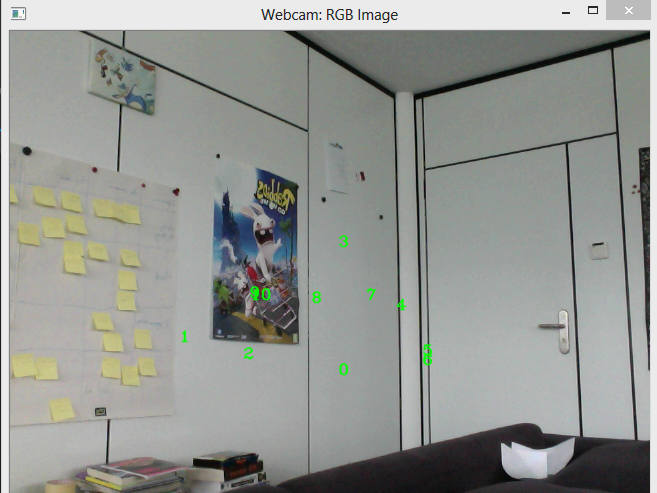
\includegraphics[scale=0.8]{images/calibration_points.png}
 	\captionof{figure}{Calibration points}
\end{center}

\begin{center}
	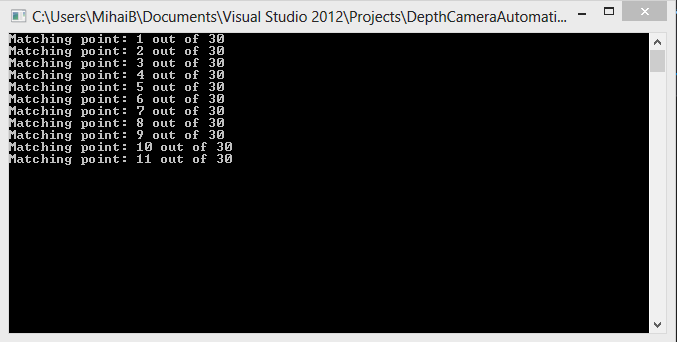
\includegraphics[scale=0.7]{images/console.png}
 	\captionof{figure}{Calibration console}
\end{center}

\begin{center}
	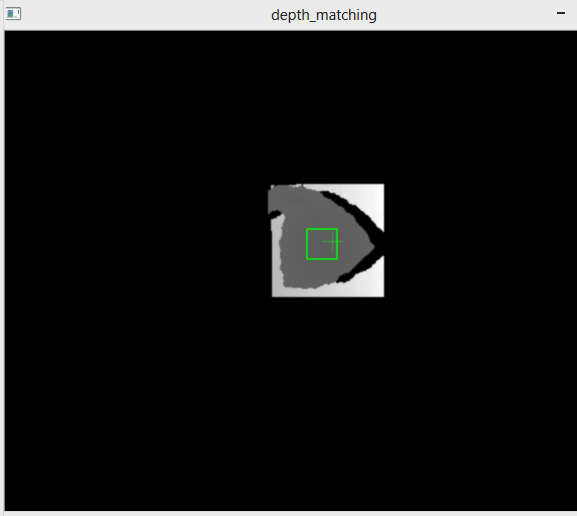
\includegraphics[scale=0.7]{images/good_kinect_depth_matching.png}
 	\captionof{figure}{Valid Kinect depth matching}
\end{center}

\begin{center}
	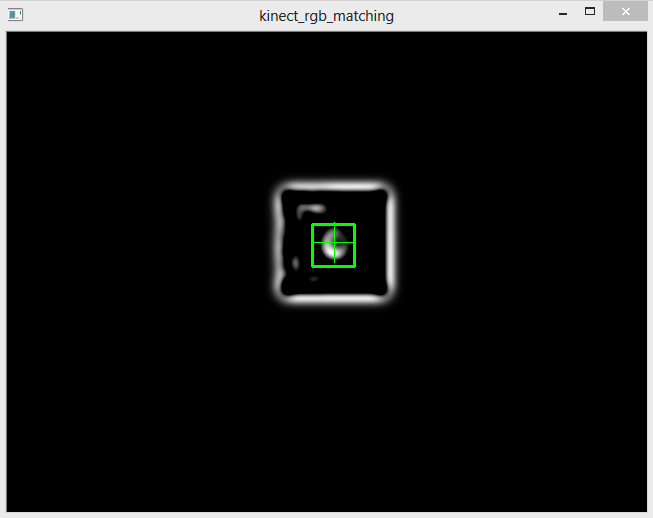
\includegraphics[scale=0.7]{images/good_kinect_rgb_matching.png}
 	\captionof{figure}{Valid Kinect RGB matching}
\end{center}

\begin{center}
	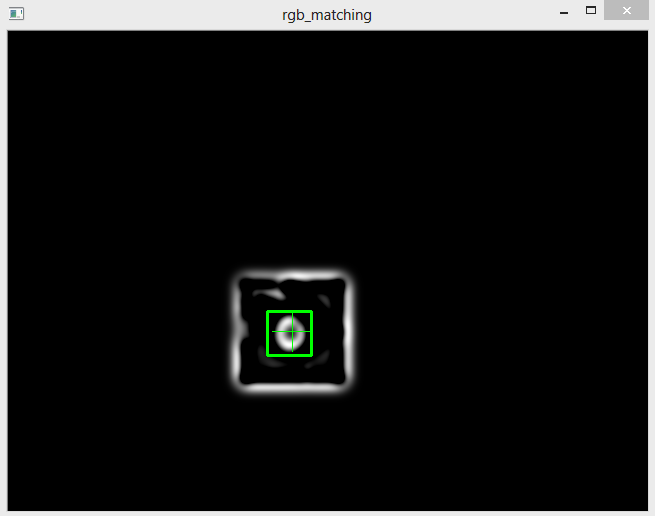
\includegraphics[scale=0.7]{images/good_rgb_matching.png}
 	\captionof{figure}{Valid webcam RGB matching}
\end{center}

\noindent
Once the calibration has been done, two new windows will appear. These windows represent the depth color reconstruction of the depth map based on the RGB image from the webcam. One window displays the image in 2D, while the other one displays the Kinect 3D point cloud. 

\begin{center}
	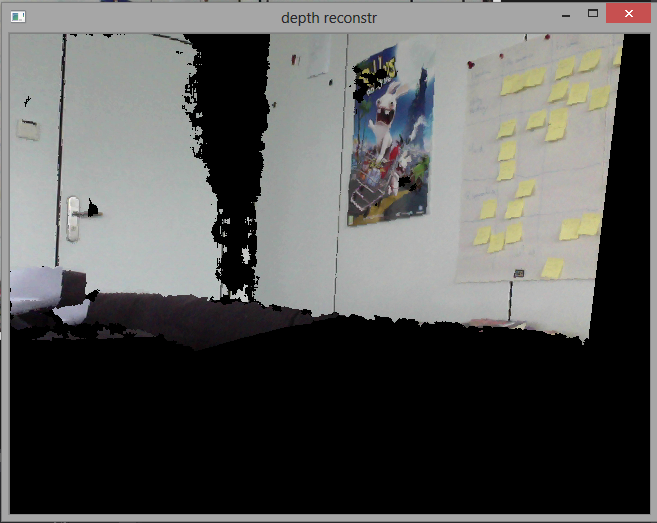
\includegraphics[scale=0.7]{images/depth_reconstruction_1.png}
 	\captionof{figure}{Depth color reconstruction}
\end{center}

\begin{center}
	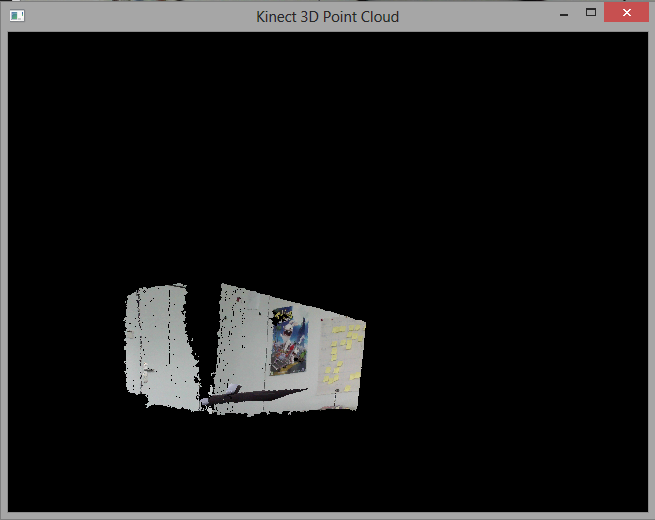
\includegraphics[scale=0.7]{images/point_cloud_1.png}
 	\captionof{figure}{Kinect 3D point cloud}
\end{center}

\begin{center}
	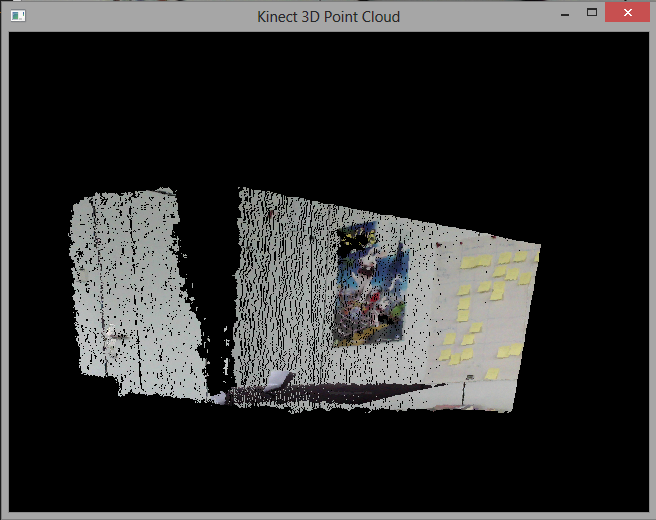
\includegraphics[scale=0.7]{images/point_cloud_2.png}
 	\captionof{figure}{Kinect 3D point cloud}
\end{center}

\begin{center}
	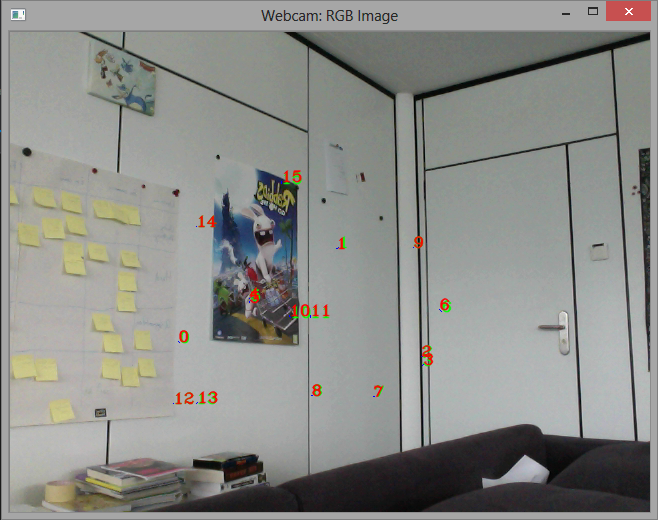
\includegraphics[scale=0.7]{images/depth_reconstruction_2.png}
 	\captionof{figure}{Reprojection of the collected points}
\end{center}

\noindent
We can also notice that the "Webcam: RGB Image" has changed. We will no longer have all the initial points, but only the points that have been kept after the iterative calibration process. We can also see the reprojections. A good calibration means that the reprojection is almost perfect, so there is no difference between the actual point detected and the point reprojected using the calibration. 

\subsection{3D point cloud scene control}
\noindent
The 3D point cloud is not just an image that one can look at. It is an environment where the user can navigate using some commands. The commands to controls the scene are described below.

\begin{itemize}
	\item w : Move in the $Z$ direction forward.
	\item a : Move in the $Z$ direction backwards.
	\item s : Strafe left ($X$ direction).
	\item d : Strafe right ($X$ direction).
	\item q : Move in the $Y$ direction up.
	\item e : Move in the $Y$ direction down.
	\item UP : Look up.
	\item DOWN : Look down.
	\item LEFT : Look left.
	\item RIGHT : Look right. 
\end{itemize}

\noindent
The controls have been made similarly to the ones found in a First Person Shooter (FPS) game. 
\\\\
\emph{Note:} For the controls to be active, the user must select the 3D point cloud window.

\section{Results}
\noindent
This section will describe the results of performing several calibrations and a comparison to the Kinect's calibration. Since we cannot test the calibration of the webcam with the calibration of the Kinect, we have performed another calibration for the Kinect. This way, we can test our calibration with the Kinect's default calibration. 

\subsection{Webcam calibration}
The minimum number of points required for a calibration is 6. However, we have seen in practice that 6 points are not enough for a good calibration. Taking into consideration that we do iterative improvement of the calibration, we need many more points since some of them will be eliminated (they are classified as outliers). One possible cause for correspondences to be considered outliers is due to the fact that the time difference between the RGB camera frame and the depth camera frame is not 0. If the pattern is quickly moving in the environment, the reprojection error might grow.  
\\\\
In practice, we have performed calibrations starting with 30 points. Once 30 points have been collected, the iterative calibration process begins. The table below shows the results that we have obtained with our calibration. 

\begin{center}
  \begin{tabular}{| c | c | c |}
    \hline
    Initial number of points & Final number of points & Calibration error \\ \hline
    30 & 18 & 2.3 \\ \hline
    30 & 12 & 2.1 \\ \hline
    30 & 8 & 2.8 \\
    \hline
  \end{tabular}
\end{center}

\noindent
The error is measured in pixels. An example of the result of the iterative calibration process can be seen below.

\begin{center}
	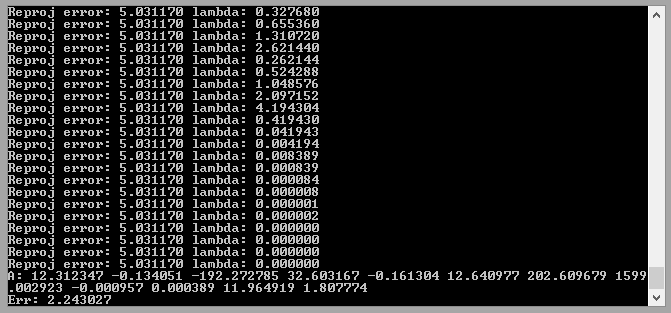
\includegraphics[scale=1]{images/webcam_calibration.png}
 	\captionof{figure}{Reprojection of the collected points}
\end{center}

\subsection{Comparison the the Kinect calibration}
\noindent
In order to compare our approach with the Kinect default calibration, we had to calibrate the Kinect. Once the Kinect has been calibrated we can compare the results of the two calibrations.
\\\\
How do we compare them?
\\\\
We take all the 3D points that have been kept in the calibrator and we reproject them on the Kinect's RGB Image. As reference points, we will consider the points that have been detected using the template matching process on the Kinect's RGB image. 

\begin{itemize}
	\item Let P3D(x,y,z) be a 3D point.
	\item We reproject P3D using our calibration and the reproject function described in the implementation. This will result in P\_ OUR(x,y).
	\item We reproject P3D using the Kinect's default calibration, using the function \emph{NuiImageGetColorPixelCoordinatesFromDepthPixelAtResolution}. We will get P\_ Kinect(x,y).
	\item We take as reference P\_ Ref(x,y) the point from the Kinect's RGB image, found using template matching.
\end{itemize}

\noindent
The goal is to be able to see which point, P\_ OUR or P\_ Kinect is closer to P\_ Ref. We have developed a visual and mathematical way to check. Some of the results that we have obtained can be seen below. 
\\\\
The mathematical way to verify the points is by computing the Euclidean distance between the target point (P\_ REF) and P\_ OUR and P\_ Kinect. The distance between them represents the error in pixels. The table below represents all the points that have been considered for a calibration, a total of 18 points. 

\begin{center}
  \begin{tabular}{| c | c | c |}
    \hline
    Id & Our Calibration Error & Kinect Calibration Error \\ \hline
    1 & 1 & 6.08276 \\ \hline
	2 & 1.41421 & 9 \\ \hline
	3 & 2 & 8.06226 \\ \hline
	4 & 1 & 8.06226 \\ \hline
	5 & 1 & 2 \\ \hline
	6 & 1 & 1.41421 \\ \hline
	7 & 1 & 2.23607 \\ \hline
	8 & 0 & 5 \\ \hline
	9 & 2.23607 & 5.38516 \\ \hline
	10 & 1 & 3 \\ \hline
	11 & 2 & 3.60555 \\ \hline
	12 & 2 & 2.82843 \\ \hline
	13 & 1 & 8.544 \\ \hline
	14 & 1.41421 & 9.05539 \\ \hline
	15 & 2 & 9.48683 \\ \hline
	16 & 1 & 7.07107 \\ \hline
  \end{tabular}
\end{center}

\begin{center}
	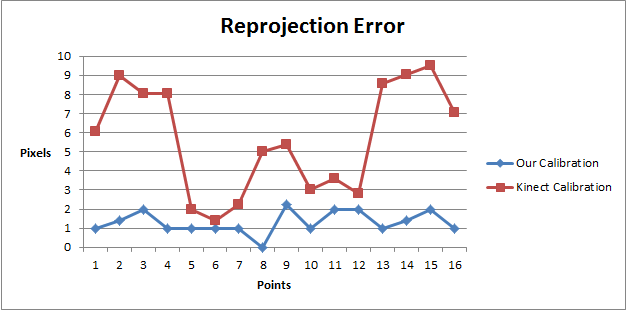
\includegraphics[scale=1]{images/chart.png}
 	\captionof{figure}{Visualization of the reprojection error}
\end{center}

\noindent
Below, you will see a series of pictures, where the points are presented in the context in which they were collected. In order to understand the comparison, each point is marked with a different color. 

\begin{itemize}
	\item \textcolor{blue}{BLUE} - The point which was detected with template matching.
	\item \textcolor{green}{GREEN} - The reprojection of the point found in the depth image using the calibration that we have developed.
	\item \textcolor{red}{RED} - The reprojection of the point found in the depth image using the calibration of the Kinect (the default calibration). 
\end{itemize}

\begin{center}
	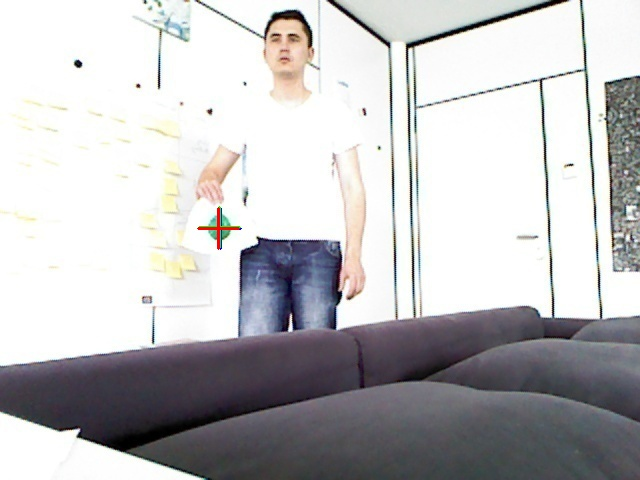
\includegraphics[scale=0.6]{images/compare_output/rgb_image_1.jpg}
 	\captionof{figure}{Reprojection of the collected points}
\end{center}

\begin{center}
	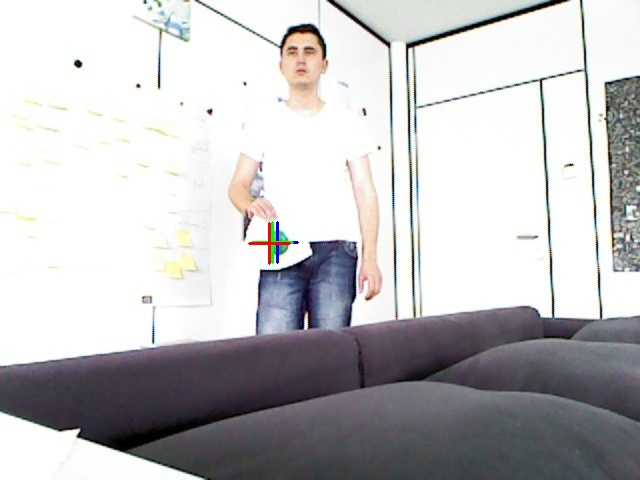
\includegraphics[scale=0.6]{images/compare_output/rgb_image_2.jpg}
 	\captionof{figure}{Reprojection of the collected points}
\end{center}

\begin{center}
	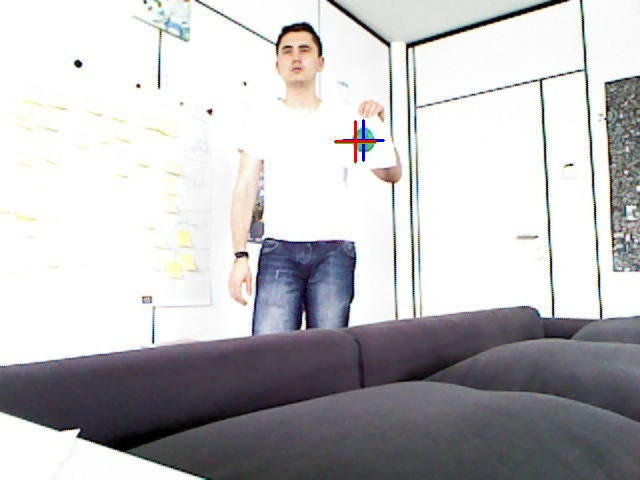
\includegraphics[scale=0.6]{images/compare_output/rgb_image_3.jpg}
 	\captionof{figure}{Reprojection of the collected points}
\end{center}

\begin{center}
	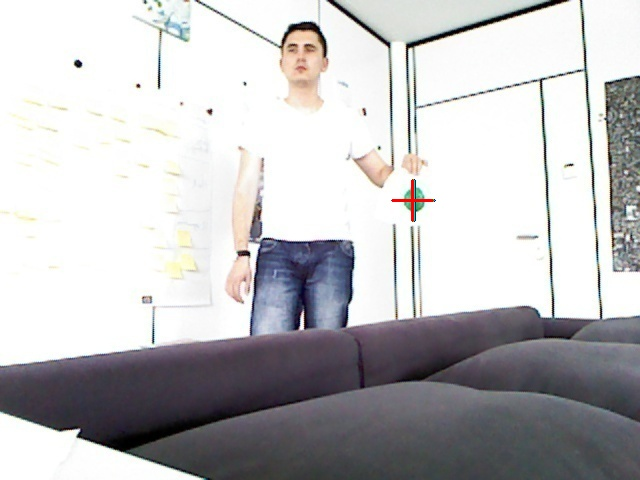
\includegraphics[scale=0.6]{images/compare_output/rgb_image_4.jpg}
 	\captionof{figure}{Reprojection of the collected points}
\end{center}

\begin{center}
	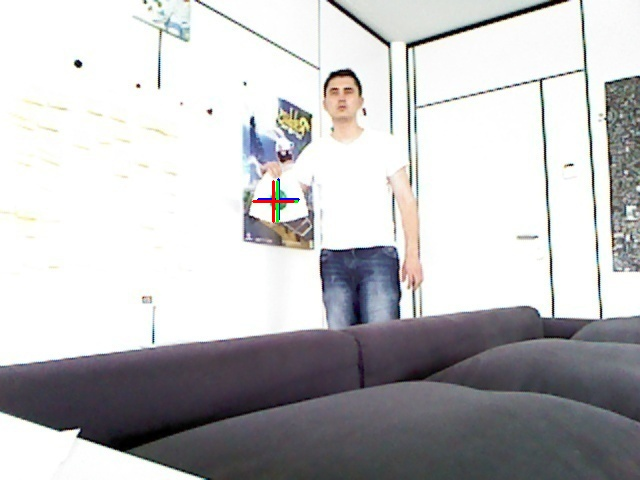
\includegraphics[scale=0.6]{images/compare_output/rgb_image_10.jpg}
 	\captionof{figure}{Reprojection of the collected points}
\end{center}

\begin{center}
	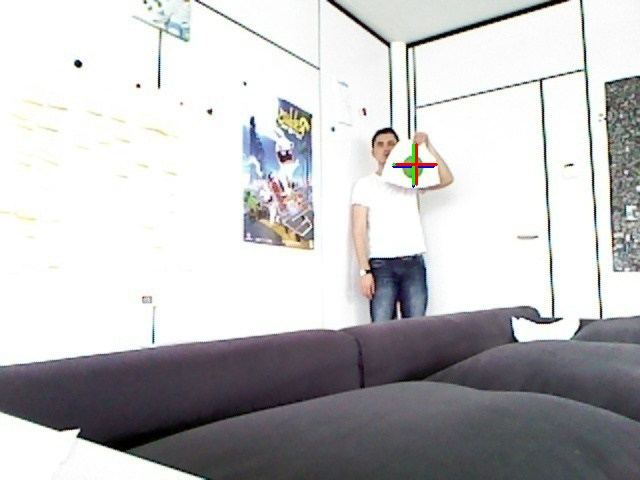
\includegraphics[scale=0.6]{images/compare_output/rgb_image_20.jpg}
 	\captionof{figure}{Reprojection of the collected points}
\end{center}

\begin{center}
	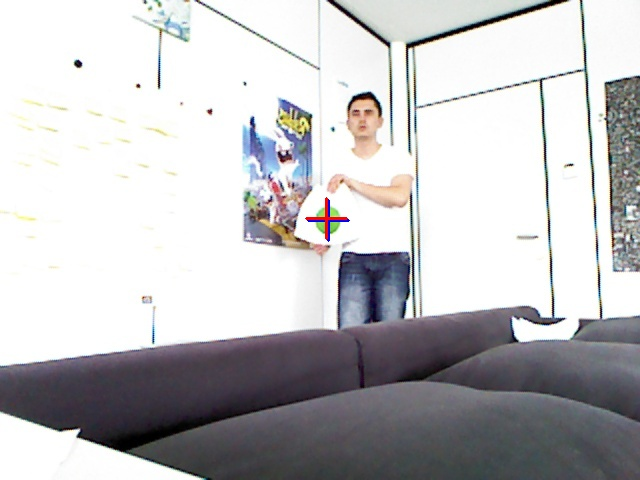
\includegraphics[scale=0.6]{images/compare_output/rgb_image_24.jpg}
 	\captionof{figure}{Reprojection of the collected points}
\end{center}

\begin{thebibliography}{9}

\bibitem{a}
  Zhengyou Zhang,
  \emph{A Flexible New Technique for Camera Calibration}.
  Microsoft Research, One Microsoft Way, Redmond, WA 98052-6399, USA
  
\bibitem{b}
	OpenCV Documnetation,
	\url{http://docs.opencv.org/}
	
\bibitem{c}
	OpenGL Documnetation,
	\url{http://www.opengl.org/documentation/}	
	
\bibitem{d}
	OpenGL Camera Part 3,
	\url{http://www.swiftless.com/tutorials/opengl/camera3.html},
	Swiftless Tutorials, Game Programming and Computer Graphics Tutorials	
	
\bibitem{e}
	Microsoft Kinect SDK documnetation,
	\url{http://msdn.microsoft.com/en-us/library/hh855366.aspx},
	MSDN Natural User Interface
	
\bibitem{f}
	Edward Zhang, Kinect SDK Tutorials, 
	\url{http://www.cs.princeton.edu/~edwardz/tutorials/index.html},
	Princeton University
	
\bibitem{g}
	Jared St. Jean,
	\emph{Kinect Hacks, Tips and Tools for Motion and Pattern Detection},
	O'REILLY
	
	

\end{thebibliography}
\addcontentsline{toc}{chapter}{Bibliography}

\end{document}